%! TEX root = diffusr.tex

\begin{table}[htb]
  \caption{Dataset statistics: number of transactions
$\protect\card{\odataset}$, number of items $\protect\card{\items}$,
density $\sfrac{\text{avg} \protect\card{t}}{\protect\card{\items}}$, where
  $\text{avg}\protect\card{t}$ is the average transaction length, sum
  $\sumtlen \doteq \sum_{i=1}^m \protect\card{t_i}$ of transaction
  lengths, support threshold $\thresh$ used in some experiments, and number of
frequent itemsets w.r.t.\ $\thresh$.}\label{tab:datasets}
  {\small
  \begin{tabular}{lrrrrrr}
    Dataset $\odataset$ & $\card{\odataset}$ & $\card{\items}$ &
    $\frac{\text{avg}\card{t}}{\card{\items}}$ & $\sumtlen$ & $\thresh$ &
    $\card{\fis{\thresh}{\odataset}}$ \\
    \midrule
    \textsc{Foodmart} & 4,141 & 1,559 & 0.0028 & 18,319 & 2 & 4,247\\
    \textsc{Chess} & 3,196 & 75 & 0.4933 & 118,252 & 2,557 & 8,227\\
    \textsc{Mushroom} & 8,416 & 119 & 0.1933 & 193,568 & 2,525 & 2,587\\
    \textsc{BMS 1} & 59,602 & 497 & 0.0051 & 149,639 & 60 & 3,991 \\
    \textsc{BMS 2} & 77,512 & 3,340 & 0.0014 & 358,278 & 156 & 3,683 \\
  \end{tabular}
  } % small
\end{table}

\section{Experimental evaluation}\label{sec:exper}

Our experimental evaluation focuses on three aspects. First, verify the presence
of the \emph{distortion} in the dataset null space $\nullset$ by looking at the
distribution of $\copiesnum{\mattodat{M}}$ across the matrices state space
$\matrices$, and assess the impact of such distortion on testing data mining
results. Second, evaluate the \emph{speed and scalability} of \algo\ by
measuring the \textit{step time} of \algo, i.e., the time to take a step on the
Markov chain, and how it changes as the number $\card{\odataset}$ of
transactions in the datasets grows. Third, empirically estimate the \emph{mixing
time} of \algo, i.e., the number of swaps for the distribution of the chain
state to be close to the stationary distribution.

\paragraph{Implementation, environment, datasets}
We implement \algo\ and \gioalgo\ in Java 8. All our code, together with
instructions and a script to reproduce all our results and figures, is available
from \url{https://anonymous.4open.science/r/DiFfuSR-KDD/}. We run our
experiments on an x86--64 AWS EC2 instance with the Amazon Linux 2 OS, 128GB of
RAM, and 32 vCPUs. We use five publicly
available\footnote{\url{https://www.philippe-fournier-viger.com/spmf/index.php?link=datasets.php}}
datasets, whose relevant statistics are in \cref{tab:datasets}. %:
% 20220131 MR: commenting out as it is not entirely needed: people know about
% these datasets. We will uncomment the following in an extended version or
% thesis.
%\begin{itemize}
%  \item \textsc{Foodmart}: customer transactions from a retail store, obtained
%    and transformed from SQL-Server 2000.
%  \item \textsc{Chess}: a conversion of the UCI chess dataset.
%  \item \textsc{Mushroom}: a conversion of the UCI mushroom dataset.
%  \item \textsc{BMS WebView 1 (BMS 1)}: click-stream data from a webstore used
%    in KDD-Cup 2000, which has been prepared for itemset miningConvergence .
%  \item \textsc{BMS WebView 2 (BMS 2)}: click-stream data from a webstore used
%    in KDD-Cup 2000, which has been prepared for itemset mining.
%\end{itemize}

\begin{table}[htb]
  \caption{Distortion: minimum, 1\textsuperscript{st} quartile, median,
    3\textsuperscript{rd} quartile, and maximum of
    $\lfloor\ln(\copiesnum{\mattodat{M}})\rfloor$ across 10,000 states $M \in
\matrices$.}\label{tab:distortion}
  {\small
  \begin{tabular}{lrrrrr}
    & \multicolumn{5}{c}{Distribution of $\lfloor \ln(\copiesnum{\mattodat{M}})
    \rfloor$} \\
    \cmidrule(lr){2-6}
    Dataset & min. & Q1 & med. & Q3 & max. \\
    \midrule
    \textsc{Foodmart} & 21,848 & 21,851 & 21,852 & 21,855 & 21,861 \\
    \textsc{Chess} & 22,589 & 22,596 & 22,598 & 22,598 & 22,599 \\
    \textsc{Mushroom} & 67,449 & 67,580 & 67,628 & 67,639 & 67,649 \\
    \textsc{BMS 1} & 343,570 & 345,695 & 347,551 & 349,260 & 350,721 \\
    \textsc{BMS 2} & 541,598 & 542,301 & 542,926 & 543,515 & 544,058
  \end{tabular}
  } % small
\end{table}

\paragraph{Distortion}
As discussed in \cref{sec:gionis}, the distortion in which \gioalgo\ incurs is
due to the fact that not every dataset $\dataset$ has the same number
$\copiesnum{\dataset}$ of matrices $M \in \matrices$ such that
$\dataset=\mattodat{M}$, or equivalently, that $\copiesnum{\mattodat{M}}$ is not
the same for every $M \in \matrices$. We verify the presence of this distortion
by performing a (non-covering) random walk over $\matrices$ and tracking the
value $\ln(\copiesnum{\mattodat{M}})$ for each visited state $M$. While a random
walk may visit a state more than once, it never happened in our experiments.
Additionally, the random walk bias towards higher-degree states has no influence
on verifying the presence of distortion. In \cref{tab:distortion} we report
quartiles of the observed distribution over 10,000 steps, without the decimal
part due to lack of space. The results show the clear presence of distortion,
given the large variability in $\copiesnum{\mattodat{M}}$.

\paragraph{Impact of distortion} \algo\ is a drop-in replacement for \gioalgo\
to validate data mining results as described by
\citet{HamalainenW19,GionisMMT07}, but the two approaches sample from two
different null models: SLISP \textit{with} distortion (\gioalgo), and
\textit{without} (\algo). Thus, it is not surprising that the outcome of the
results validation may differ, depending on which method is used, and therefore
which null model is assumed. To keep the presentation focused, and due to space
constraints, we briefly discuss here a few results on the impact of distortion
on validating data mining results, and defer a full evaluation to the extended
version. We tested the significance of the number
$\card{\fis{\thresh}{\odataset}}$ of frequent patterns (see
\cref{sec:prelims:significant}), using 2,048 sample datasets for each method to
approximate the null distribution of this statistic. Not surprisingly (as
discussed above), using \gioalgo\ or \algo\ results different empirical null
distributions, which could lead to different $p$-values and hence to different
outcomes of the test depending on the critical value. In our preliminary
analysis using \algo\ for significant frequent itemset
mining~\citep{HamalainenW19,PellegrinaRV19b}, we observed that the set of
significant patterns found by \gioalgo\ in the \textsc{Chess} dataset with FWER
$\delta=0.05$,  was extremely different (Jaccard index: 0.12) from the sets of
significant patterns found by the two \algo\ methods. Once more, this result is
evidence that the user must be extremely cautious in choosing the method and
therefore the assumed null model: the meaning of significance depends on the
null model, and comparing results obtained under different null models (e.g., to
compare the statistical power of two procedures) has no meaning.

\begin{table}[htb]
  \caption{Step time (in ms): minimum, 1\textsuperscript{st} quartile,
  median, 3\textsuperscript{rd} quartile, and maximum over 10,000
  steps.}\label{tab:steptimes}
  {\small
  \begin{tabular}{llrrrrr}
    & & \multicolumn{5}{c}{step time (ms)} \\
    \cmidrule(lr){3-7}
    Dataset & algorithm & min. & Q1 & med. & Q3 & max. \\
    \midrule
    \multirow{3}{*}{\textsc{Foodmart}} & \naivealgo\ & $<1$ & 1 & 2 & 2 & 16 \\
    & \refalgo\ & 1 & 2 & 2 & 2 & 32 \\
    & \gioalgo\ & 1 & 1 & 2 & 2 & 24 \\
    \midrule
    \multirow{3}{*}{\textsc{Chess}} & \naivealgo\ & 4 & 5 & 5 & 5 & 24 \\
    & \refalgo\ & 11 & 13 & 14 & 14 & 49 \\
    & \gioalgo\ & 3 & 5 & 5 & 5 & 16 \\
    \midrule
    \multirow{3}{*}{\textsc{Mushroom}} & \naivealgo\ & 8 & 12 & 13 & 13 & 56 \\
    & \refalgo\ & 22 & 28 & 30 & 33 & 82 \\
    & \gioalgo\ & 7 & 9 & 9 & 10 & 47 \\
    \midrule
    \multirow{3}{*}{\textsc{BMS 1}} & \naivealgo\ & 19 & 25 & 27 & 29 & 63 \\
    & \refalgo\ & 27 & 31 & 32 & 38 & 73 \\
    & \gioalgo\ & 19 & 24 & 25 & 27 & 63 \\
    \midrule
    \multirow{3}{*}{\textsc{BMS 2}} & \naivealgo\ & 33 & 44 & 47 & 50 & 98 \\
    & \refalgo\ & 50 & 55 & 56 & 57 & 103 \\
    & \gioalgo\ & 38 & 47 & 49 & 51 & 97
  \end{tabular}
  } % small
\end{table}

\begin{figure}[htb]
  \centering
  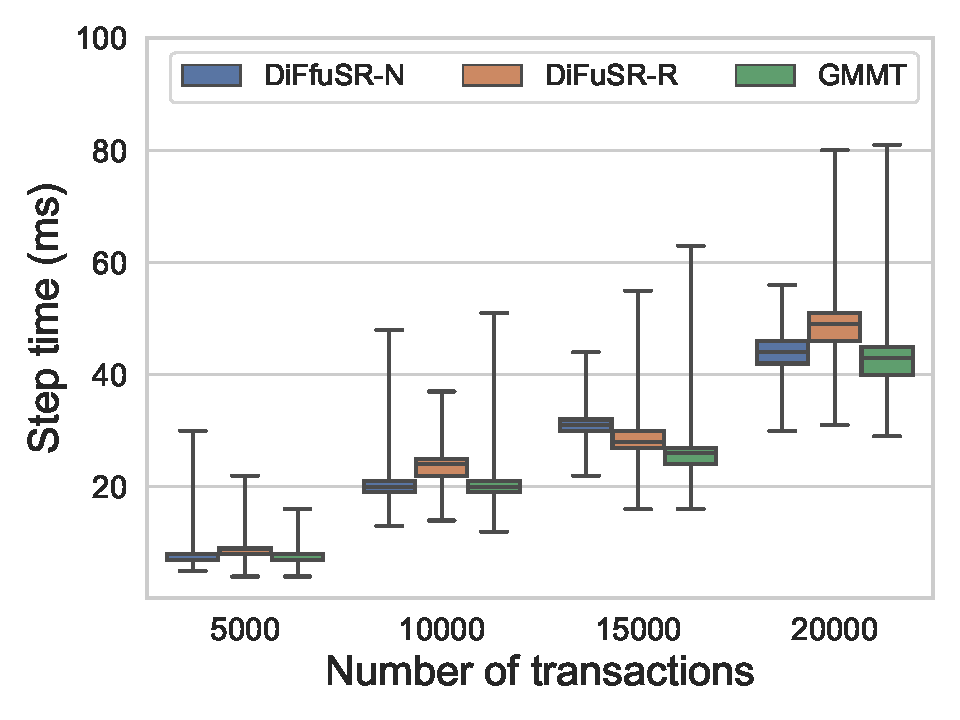
\includegraphics[width=.4\textwidth,height=110pt]{scalability.pdf} % chktex 8
  \caption{Scalability results: The step time distribution (in milliseconds)
    over 10,000 swaps for increasing values of $\protect\card{\odataset}$. The
    line in each box corresponds to the median, the bottom and top of each box
    correspond to the first and third quartiles, and the lower and upper
    whiskers correspond to the minimum and maximum.}\label{fig:scalability}
  \Description{Scalability results.}
\end{figure}%

\begin{figure*}[tb]
  \centering
  \begin{subfigure}{0.33\textwidth}
    \centering
    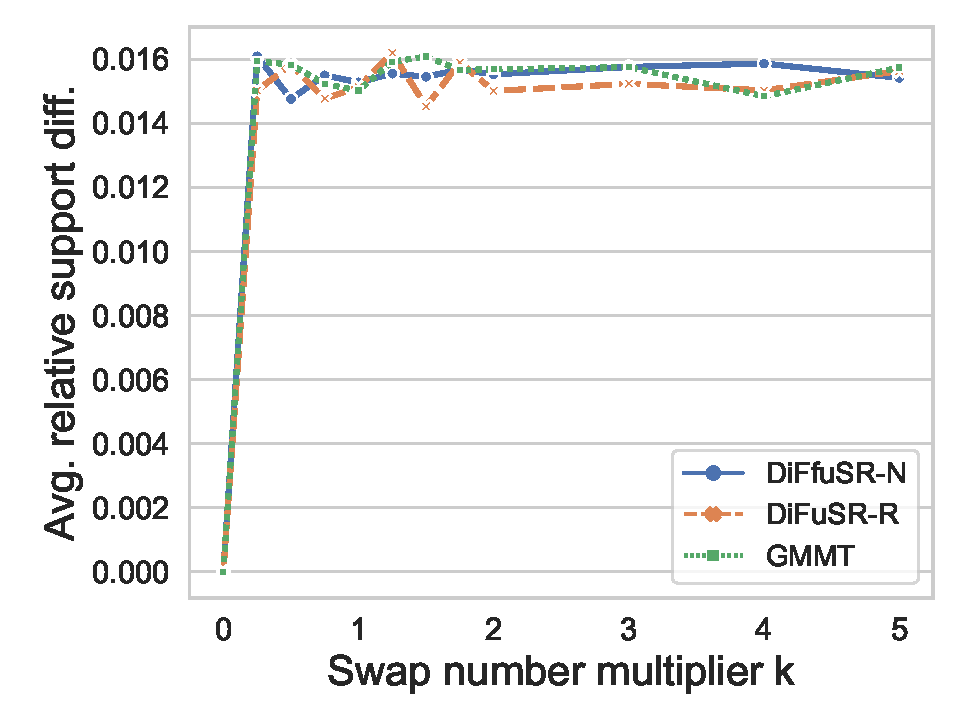
\includegraphics[width=\textwidth,height=105pt]{convergence-chess-5-0.8-0.pdf} % chktex 8
    \caption{\textsc{Chess}}\label{fig:arsdchess}
  \end{subfigure}%
  \begin{subfigure}{0.33\textwidth}
    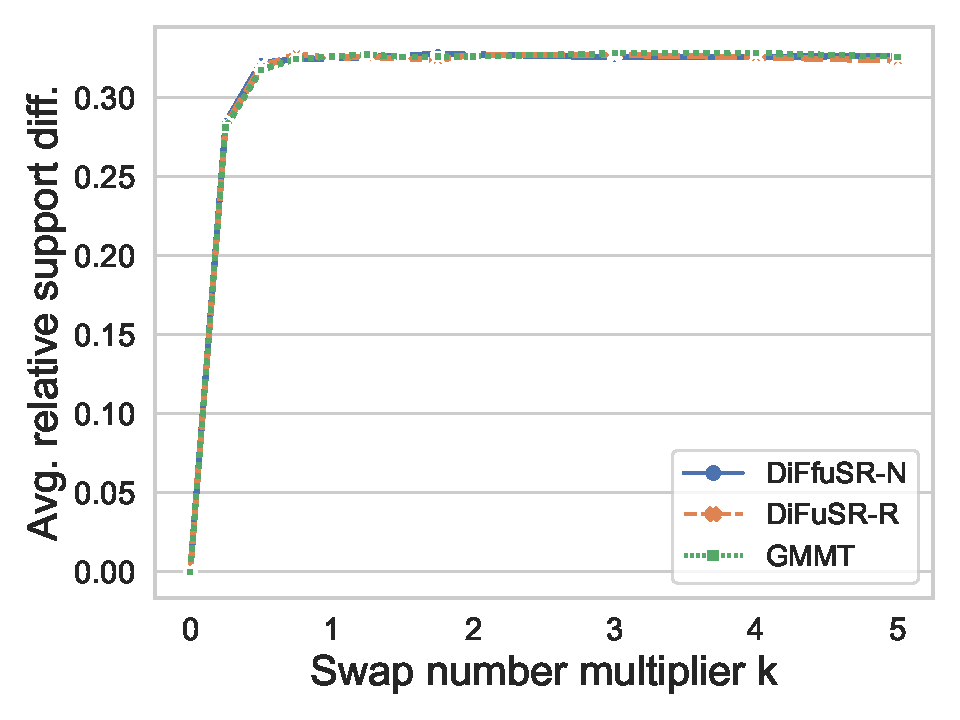
\includegraphics[width=\textwidth,height=105pt]{convergence-mushrooms-5-0.3-0.pdf} % chktex 8
    \caption{\textsc{Mushroom}}
  \end{subfigure}%
  \begin{subfigure}{0.33\textwidth}
    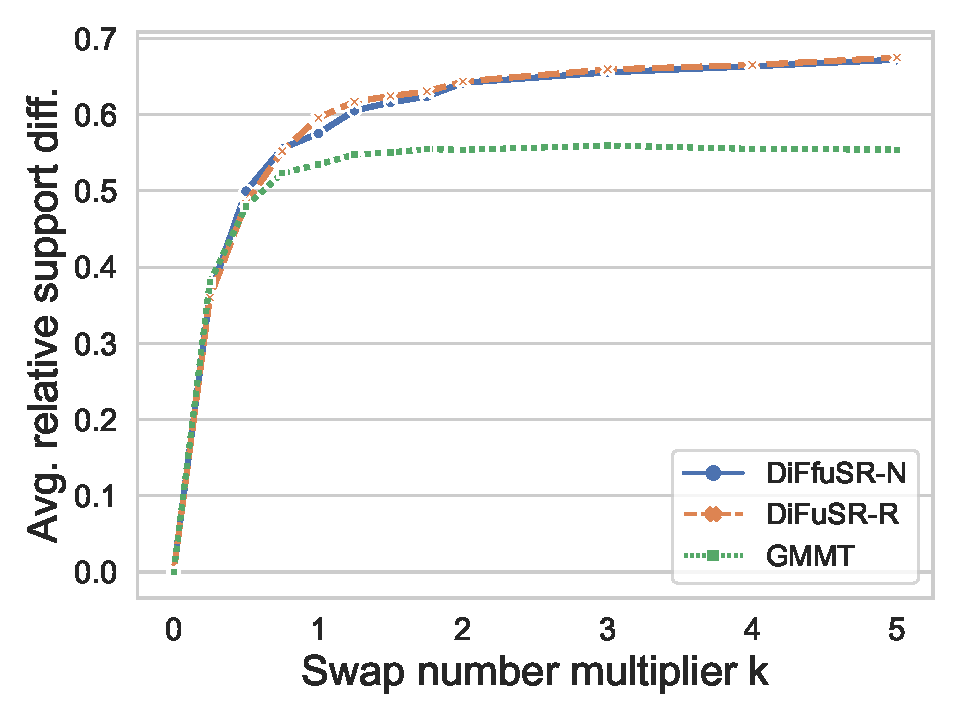
\includegraphics[width=\textwidth,height=105pt]{convergence-BMS1-5-0.001-0.pdf} % chktex 8
    \caption{\textsc{BMS 1}}
  \end{subfigure}
  \caption{Convergence results: $\arsd{\odataset}$ as the swap number multiplier
    $\swapnummult$ grows, where $\swapnummult$ is s.t.\ the number of swaps is
    $\swapnum \doteq \lfloor \swapnummult \sum_{i=1}^m
  \protect\card{t_i}\rfloor$.}\label{fig:arsd}
  \Description{Convergence results.}
\end{figure*}

\paragraph{Step times}
The \emph{step time} is the time needed to obtain a valid swap, compute the MH
acceptance probability, and transition to the next state if it is accepted. In
\cref{tab:steptimes} we report the distribution, over 10,000 steps, of this
quantity. We show the results for \gioalgo\ \emph{only} for comparison purposes:
due to the distortion it incurs, \gioalgo\ is not to be preferred just because
it appears faster.

The distribution for \naivealgo\ is comparable to that of \gioalgo, while
\refalgo\ is slightly slower. This is expected since the execution of
\gioalgo\ and \naivealgo\ are very similar, where the only additional work for
\naivealgo\ is to compute $\copiesnum{\mattodat{M''}}$ from
$\copiesnum{\mattodat{M'}}$. \refalgo\ is slower because it needs to
compute $\selfspairsnum{\dataset''}$ from $\selfspairsnum{\dataset'}$, which
takes time linear in the numbers of transactions with the same lengths as the
ones involved in the swaps (\cref{algline:tlloop} of \cref{algo:getselfspairsnumneigh}).
For this same reason, \refalgo\ is relatively slower than the others on datasets
where every transaction has the same length (\textsc{Chess}, \textsc{Mushroom}).

\paragraph{Scalability}
We use the IBM Quest generator to create synthetic datasets with
$\card{\odataset} \in \{$5,000, 10,000, 15,000, 20,000$\}$, on
$\card{\items}=100$ and average transaction length $\card{t}=25$. We run all
algorithms for 10,000 swaps on each dataset, and report the results in
\cref{fig:scalability}.

There is a linear relationship between the distribution of step times and the
number of transactions, as all algorithms need to compute
$\totspairsnummat{M_{\dataset''}}$, which takes time linear in
$\card{\dataset''}$. The interquartile range ($Q3 - Q1$) grows in absolute
terms because the individual step times grow, but it is essentially constant in
relative terms.

\paragraph{Convergence to the stationary distribution}
Since we cannot prove an upper bound to the mixing time of the Markov chains
used by our algorithms (see \cref{sec:extensions}), we empirically estimate it.
Following other works using MCMC with MH for swap
randomization~\citep{TononV19}, we estimate the mixing time by tracking the
\emph{Average Relative Support Difference (ARSD)}, defined as follows. Given the
observed dataset $\odataset$, let $\thresh \in \lparen0,\card{\odataset}\rbrack$
be a minimum support threshold, and $\dataset_\swapnum$ be the dataset
corresponding to the state of the chain after $\swapnum \in \mathbb{N}$ swaps.
Then, the average relative support difference $\arsd{\dataset_\swapnum}$ of
$\dataset_\swapnum$ is
\[
  \arsd{\dataset_\swapnum} \doteq \frac{1}{\card{\fis{\thresh}{\odataset}}}
  \sum_{A \in \fis{\thresh}{\odataset}} \frac{\abs{\supp{A}{\odataset} -
  \supp{A}{\dataset_\swapnum}}}{\vphantom{\supp{A}{\nonsmashedodataset}}\supp{A}{\odataset}} \enspace.
  % vphantom for pretty printing
\]
In \cref{fig:arsd,fig:addarsd} (in \cref{sec:addarsd}) we report
$\arsd{\dataset_\swapnum}$ for $\swapnum \doteq \lfloor \swapnummult \sumtlen
\rfloor$ swaps, where $\swapnummult \in \{0, 0.25, 0.50, \dotsc, 2, 3, 4, 5\}$
and $\sumtlen \doteq \sum_{i = 1}^{m} \card{t_i}$, for each dataset. We use the
values of $\thresh$ from \cref{tab:datasets}:  the qualitative results do not
change with other values.

We remark that comparing the mixing times of Markov chains with different
stationary distributions (as \gioalgo\ and \naivealgo) and even on different
sets of states (as \refalgo\ vs.\ the other two) is \emph{meaningless}, as they
allow to sample different objects from different sets according to different
distributions. Neither are the values of the ARSD comparable, as they are
\emph{proxies} for the mixing times, but not for the distance between the state
distribution and the stationary distribution, and they also depend on the chosen
$\thresh$. Therefore, we do not make such comparisons and only include the
results from \gioalgo\ for completeness (the mixing time for
\gioalgo\ is the same observed by \citet[Sect.\ 5.1]{GionisMMT07}).

\Cref{fig:arsd,fig:addarsd} (in \cref{sec:addarsd}) show that in all cases, the
ARSD stabilizes by $\swapnum = 2 \sumtlen$ swaps or earlier (by $\swapnum =
\sumtlen$), i.e., the mixing time appears to be linear in $\sumtlen$. For
\textsc{Chess}, the fluctuations in the ARSD may seem large due to the scale of
the y-axis, which is much smaller in \cref{fig:arsdchess} than in the other
subfigures.
